\documentclass[sigconf,review,anonymous]{acmart}

\usepackage{amsmath}
\usepackage{booktabs}
\usepackage{multirow}
\usepackage{algorithm}
\usepackage[noend]{algpseudocode}
\usepackage{graphicx}
\usepackage{xcolor}
\usepackage{tikz}
\usetikzlibrary{arrows.meta,positioning}

\newcommand{\system}{\textsc{ML-UNG}}
\newcommand{\ung}{\textsc{UNG}}
\newcommand{\pending}[1]{\textcolor{red}{[pending: #1]}}
\newcommand{\dataset}{\mathcal{D}}
\newcommand{\labels}{\mathcal{A}}
\newcommand{\eligible}{\mathcal{E}}
% This file is intentionally kept separate from main.tex.
% The authoritative result generator will replace this text only after the
% screen, crossing, formal, profile, held-out, and build validators pass.

\subsection{Query Performance}
\pending{Authoritative formal results are still running.}

\subsection{Automatic Versus Manual Hierarchies}
\pending{Report per-workload oracle regret, global-configuration regret, and
held-out results.}

\subsection{Mechanism Breakdown}
\pending{Report stage timing and search-work counters from the profile pass.}

\subsection{Construction}
\pending{Report repeated end-to-end CPU/GPU builds, resource use, index size,
and downstream search-quality checks.}

\newcommand{\baseTopologyFactorialTables}{%
\begin{table*}[t]
\centering\scriptsize
\caption{Zero- and one-overlay configurations in the complete Amazon base-by-overlay topology screen at Recall@10 $\geq0.90$. A code $m$L[$B|U$] lists base topology $B$ before the separator and upper topologies $U$ from fine to coarse. $L$ is LNG and $T$ is Trie. The base uses its matched entry provider: optimized-LNG for $B=L$ and Trie for $B=T$. NC$(r)$ gives maximum minimum-warm-repeat Recall when there is no crossing in the shared measured budget.}
\label{tab:base-topology-factorial-a}
\resizebox{\textwidth}{!}{%
\begin{tabular}{rrrrrrr}
\toprule
Sel. & 0L[L] & 0L[T] & 1L[L|L] & 1L[L|T] & 1L[T|L] & 1L[T|T] \\
\midrule
0.499\% & 2476.35 & 14921.90 & NC (0.888) & NC (0.888) & 15177.24 & 17937.69 \\
0.903\% & 4191.04 & 11591.42 & NC (0.857) & NC (0.846) & 12447.15 & 12144.74 \\
5.038\% & 544.93 & 10044.23 & NC (0.893) & NC (0.883) & 9105.22 & 10937.27 \\
9.907\% & 450.17 & 270.63 & NC (0.874) & NC (0.848) & 289.73 & 146.19 \\
30.027\% & 52.77 & NC (0.888) & NC (0.836) & NC (0.828) & 27.66 & 10.50 \\
60.047\% & 4.07 & 2.51 & 56.52 & 56.70 & 1613.68 & 839.32 \\
80.024\% & 1.80 & 0.59 & 36.65 & 37.08 & 648.35 & 285.42 \\
95.020\% & 1.50 & 0.49 & 42.06 & 36.82 & 520.35 & 265.13 \\
99.001\% & 0.79 & 0.44 & 15.40 & 14.34 & 253.23 & 264.44 \\
\bottomrule
\end{tabular}
}
\end{table*}
\begin{table*}[t]
\centering\scriptsize
\caption{Two-overlay configurations in the complete Amazon base-by-overlay topology screen at Recall@10 $\geq0.90$. A code $m$L[$B|U$] lists base topology $B$ before the separator and upper topologies $U$ from fine to coarse. $L$ is LNG and $T$ is Trie. The base uses its matched entry provider: optimized-LNG for $B=L$ and Trie for $B=T$. NC$(r)$ gives maximum minimum-warm-repeat Recall when there is no crossing in the shared measured budget.}
\label{tab:base-topology-factorial-b}
\resizebox{\textwidth}{!}{%
\begin{tabular}{rrrrrrrrr}
\toprule
Sel. & 2L[L|LL] & 2L[L|LT] & 2L[L|TL] & 2L[L|TT] & 2L[T|LL] & 2L[T|LT] & 2L[T|TL] & 2L[T|TT] \\
\midrule
0.499\% & NC (0.888) & NC (0.888) & NC (0.888) & NC (0.888) & 19158.52 & 21707.89 & 20593.10 & 17565.42 \\
0.903\% & NC (0.857) & NC (0.857) & NC (0.846) & NC (0.846) & 13242.16 & 14278.50 & 14062.30 & 12353.41 \\
5.038\% & NC (0.893) & NC (0.893) & NC (0.884) & NC (0.884) & 9569.96 & 11718.35 & 11082.17 & 10046.26 \\
9.907\% & NC (0.848) & NC (0.849) & NC (0.822) & NC (0.823) & 270.57 & 275.64 & 135.16 & 139.26 \\
30.027\% & NC (0.839) & NC (0.839) & NC (0.833) & NC (0.832) & 24.92 & 25.42 & 27.05 & 27.14 \\
60.047\% & 56.37 & 61.40 & 57.00 & 56.42 & 1565.04 & 1598.42 & 849.99 & 844.65 \\
80.024\% & 35.44 & 49.70 & 35.88 & 35.94 & 647.95 & 646.83 & 305.37 & 313.61 \\
95.020\% & 39.61 & 39.75 & 36.99 & 36.68 & 451.32 & 564.63 & 267.67 & 269.48 \\
99.001\% & 14.69 & 16.79 & 14.41 & 14.28 & 253.95 & 257.77 & 265.85 & 267.67 \\
\bottomrule
\end{tabular}
}
\end{table*}
}
\newcommand{\baseTopologyFactorialFindings}{%
\paragraph{Complete base-by-overlay factorial.}
The workload-wise oracle selects \texttt{2L[T|LT]} at 0.5\%, 1\%, 5\%, and 95\%; \texttt{0L[L]} at 10\% and 30\%; \texttt{1L[T|L]} at 60\% and 80\%; and \texttt{2L[T|TT]} at 99\%.  Thus no static topology dominates every workload. Among configurations crossing the Recall target at all nine selectivities, \texttt{2L[T|LT]} ranks first by geometric mean of QPS normalized to the per-workload oracle (0.868), but its worst fraction of the oracle is 0.482, at 30\%.  The matched-provider base-only comparison is equally non-monotone: \texttt{0L[T]} is 6.03$\times$, 2.77$\times$, and 18.43$\times$ faster at 0.5\%, 1\%, and 5\%, respectively, but is 0.60$\times$ at 10\%, does not cross at 30\% ($R_{\max}=0.8882$), and is 0.62$\times$--0.33$\times$ at 60\%--95\% (0.56$\times$ at 99\%).  These are end-to-end system ratios because the two bases use different compatible entry providers.

The controlled upper-level comparisons reveal a more stable role for Trie. With a Trie base and LNG at level 1, changing only level 2 from LNG to Trie (\texttt{2L[T|LL]}$\rightarrow$\texttt{2L[T|LT]}) improves QPS in eight of nine workloads, by up to 1.251$\times$; the remaining 80\% point is effectively tied at 0.998$\times$.  In contrast, changing only the finer level 1 from LNG to Trie with level 2 fixed to LNG wins in five of nine workloads but loses 40.7\%--52.9\% at 10\%, 60\%, 80\%, and 95\%.  The evidence therefore favors Trie as a sparse coarse overlay more consistently than as the fine navigation topology, while retaining an LNG fallback for the 10\%--30\% region.

\begin{table*}[t]
\centering\small
\caption{Best measured configuration at each Amazon selectivity.  Each depth column is optimized only within that depth; the overall column ranges over all 14 configurations.  Values are QPS at Recall@10 $\geq0.90$.}
\label{tab:base-topology-winners}
\begin{tabular}{r rr rr rr rr}
\toprule
Sel. & \multicolumn{2}{c}{Overall} & \multicolumn{2}{c}{Best 0L} & \multicolumn{2}{c}{Best 1L} & \multicolumn{2}{c}{Best 2L} \\
 & Config. & QPS & Config. & QPS & Config. & QPS & Config. & QPS \\
\midrule
0.5\% & 2L[T|LT] & 21707.89 & 0L[T] & 14921.90 & 1L[T|T] & 17937.69 & 2L[T|LT] & 21707.89 \\
0.9\% & 2L[T|LT] & 14278.50 & 0L[T] & 11591.42 & 1L[T|L] & 12447.15 & 2L[T|LT] & 14278.50 \\
5.0\% & 2L[T|LT] & 11718.35 & 0L[T] & 10044.23 & 1L[T|T] & 10937.27 & 2L[T|LT] & 11718.35 \\
9.9\% & 0L[L] & 450.17 & 0L[L] & 450.17 & 1L[T|L] & 289.73 & 2L[T|LT] & 275.64 \\
30.0\% & 0L[L] & 52.77 & 0L[L] & 52.77 & 1L[T|L] & 27.66 & 2L[T|TT] & 27.14 \\
60.0\% & 1L[T|L] & 1613.68 & 0L[L] & 4.07 & 1L[T|L] & 1613.68 & 2L[T|LT] & 1598.42 \\
80.0\% & 1L[T|L] & 648.35 & 0L[L] & 1.80 & 1L[T|L] & 648.35 & 2L[T|LL] & 647.95 \\
95.0\% & 2L[T|LT] & 564.63 & 0L[L] & 1.50 & 1L[T|L] & 520.35 & 2L[T|LT] & 564.63 \\
99.0\% & 2L[T|TT] & 267.67 & 0L[L] & 0.79 & 1L[T|T] & 264.44 & 2L[T|TT] & 267.67 \\
\bottomrule
\end{tabular}
\end{table*}
}


\title{\system: Metadata-Aware Multilevel Graph Navigation for Calibration-Free Filtered Approximate Nearest-Neighbor Search}

\begin{document}

\begin{abstract}
Filtered approximate nearest-neighbor search must reconcile vector proximity
with metadata predicates.  Unified Navigating Graph (UNG)~\cite{cai2024ung}
supports containment predicates by grouping vectors with identical label sets
and connecting these groups through a label navigating graph.  Because every
navigation unit remains an exact-label group, however, UNG exposes only one
granularity: as filter selectivity increases, a query must traverse many small
groups and cross-group edges, and its graph work approaches a full-index
search.

We present \system, which augments a configurable exact-group base graph with
independently constructed metadata-aware overlays.  The base can use UNG's LNG
or a materialized prefix-Trie topology.  At level $\ell$, a point-mass threshold
$T_\ell$ partitions compatible label-Trie subtrees into coarser blocks; each
block owns a local proximity graph, and blocks are connected by an LNG or a
prefix-Trie topology.  A query authorizes a block only when its labels are
contained in the block root.  Every search state carries an activation level
and expands only edges owned by that level; if no useful upper block is
authorized, \system invokes the unchanged level-0 base search.  The hierarchy
therefore reduces redundant fine-group traversal without weakening predicate
eligibility or mixing edges across levels.

To eliminate manual choices of overlay count and block size, Degree-Ratio
Hierarchy derives thresholds, overlay depth, topology, and a next-scale routing gate
from dataset cardinality and existing graph-degree budgets.  It requires no
query distribution, learned model, latency measurement, or Recall calibration.
We further batch irregular intra-block and cross-block construction on the GPU.
\authoritativeAbstractResult
\end{abstract}

\maketitle

\section{Introduction}
Filtered vector search returns the nearest vectors satisfying a predicate over
metadata.  For a containment query, the query supplies a set of labels and a
vector is eligible only if its label set contains every query label.  Graph
indexes for this problem must provide both geometric navigation and predicate
reachability.  The two signals do not coincide: nearby vectors may violate the
predicate, while eligible vectors may be scattered across many label sets.

\ung~\cite{cai2024ung} resolves this mismatch by introducing an explicit label
navigation plane.  It groups vectors that have identical label sets, builds a
proximity graph inside each group, connects minimal strict-superset groups with
an LNG, and realizes those group edges as vector edges.  For a containment
query, a label Trie helps locate minimal observed supersets, after which one
bounded graph search follows only predicate-compatible directions.  This is
the right starting point for our work: we retain UNG's exact groups, its
containment direction, and its unified vector-search interface, while making
the group topology an explicit design choice rather than an implicit constant.

The limitation we address is different from predicate correctness.  UNG has
one label-navigation granularity: every vertex of its LNG denotes one exact
label set.  This fine partition is useful for narrow predicates, but a broad
predicate may authorize hundreds of thousands of vectors spread over many
exact groups.  Search must still enter and traverse this fine graph.  On our
Amazon workload, the base index contains 482,387 observed groups for 602,453
vectors; at 95.02\% selectivity the measured UNG-style base search visits
451,225 vertices and scans 3.97 million edges per query
(Table~\ref{tab:amazon-profile}).  Merely replacing the LNG by a sparser graph
does not solve the problem: it can remove the containment paths needed for
Recall.

Recent SIGMOD and PVLDB systems make range-filtered search robust across query
widths by compressing, composing, or selecting among range-specialized graph
structures~\cite{zuo2024serf,xu2024irangegraph,liang2024unify,peng2025dynamic}.
Their filters live in an ordered scalar domain.  Containment over arbitrary
label sets has a different partial order: two eligible supersets need not lie
on one prefix branch, and a coarsened region is safe only when every point it
admits satisfies the whole query label set.  Our objective is therefore not to
transfer a range index, but to expose multiple safe navigation scales inside
UNG's label-containment model.

Our key observation is that containment admits \emph{safe coarse navigation}.
Suppose a node of the canonical label Trie represents prefix $R_b$.  Every
exact-label group in its subtree contains $R_b$.  Therefore, when
$Q\subseteq R_b$, all direct members of a block rooted there satisfy the query.
This gives a query-independent way to aggregate fine groups without weakening
the filter.  The resulting coarse graph is an overlay, not a replacement: the
configured exact-group graph remains available whenever no coarse block is
useful.  Our calibration-free default preserves UNG's LNG at this base, while
the complete topology factorial also measures a Trie base.

\system turns this observation into a multiscale UNG through three separable
mechanisms.  Increasing mass
thresholds independently partition the label Trie into blocks.  Each overlay
connects its blocks using either the LNG cover relation or a prefix-Trie
sparsifier.  Exact authorization selects legal overlays, while candidates carry
an activation level and expand only edges owned by that level.  We deliberately
separate this inter-block topology from entry-group discovery: UNG already
uses a Trie during entry lookup, whereas our \emph{Trie topology} means that
Trie ancestry itself defines materialized inter-block edges.  Table~\ref{tab:ung-delta}
summarizes the boundary between inherited and new mechanisms.

The hierarchy introduces a second problem: naively exposing both the number of
layers and every block threshold replaces one tuning knob with several.  We
therefore derive them with Degree-Ratio Hierarchy (DRH), a deterministic rule
based only on dataset size and the graph's existing degree budgets.  DRH never
observes query frequencies, latency, Recall, or a selectivity histogram.  A
structural mass gate decides whether a legal overlay is large enough to use;
rejected queries invoke the unchanged level-0 base search.

This paper makes the following contributions.
\begin{itemize}
  \item \textbf{Multiscale label navigation.} We extend UNG's single exact-group
  navigation plane with independently constructed, predicate-safe block
  overlays.  The exact-group partition is preserved; its topology and every
  overlay topology are explicit LNG/Trie choices, and the default policy keeps
  the UNG LNG base as a robust fallback.
  \item \textbf{Auditable query semantics.} Exact block authorization,
  level-tagged states, level-local edge expansion, and structural fallback make
  it explicit when an overlay may participate and prevent hidden cross-level
  behavior.  Topology and entry discovery remain separate experimental axes.
  \item \textbf{Calibration-free structure selection.} DRH derives overlay
  count, block thresholds, per-overlay topology, and the next-scale routing gate
  from $N$, $R$, and $C$, eliminating query-trace and performance calibration.
  \item \textbf{End-to-end evidence.} We evaluate measured equal-Recall
  crossings, expose both substantial high-selectivity gains and held-out
  regressions, and accelerate sidecar construction with batched GPU
  intra-block and cross-block primitives.  We do not infer universal dominance
  from the favorable cases.
\end{itemize}

\section{Problem Definition}
Let $\dataset=\{(x_i,A_i)\}_{i=1}^{N}$, where $x_i\in\mathbb{R}^d$ and
$A_i\subseteq\labels$ is a finite label set.  For a query vector $q$, query
labels $Q$, and result count $K$, containment filtering defines
\begin{equation}
  \eligible(Q)=\{i\mid Q\subseteq A_i\}.
\end{equation}
The exact answer is the $K$ points in $\eligible(Q)$ with minimum distance to
$q$.  We report
\begin{equation}
  \mathrm{Recall@}K = \frac{|R_K(q,Q)\cap R^*_K(q,Q)|}{K},
\end{equation}
where $R_K$ is the approximate result and $R^*_K$ is exact filtered ground
truth.

The empty label set is a valid predicate rather than a missing value:
$\eligible(\varnothing)=\dataset$.  Trie entry discovery therefore returns the
minimal terminal frontier reachable from the root.  We precompute this
frontier when the Trie is built or loaded, so an empty predicate costs
$O(|F_{\mathrm{root}}|)$ rather than a full Trie scan.  Returning no entries for
this case would change containment semantics and can silently corrupt broad
selectivity workloads.

Vectors with the same label set form a group $G_S=\{i\mid A_i=S\}$.  The
group partition is exact and disjoint.  A group topology is a directed graph
over observed label sets.  The base vector graph contains intra-group
proximity edges and vector-level realizations of the group-topology edges.

\section{From UNG to Multiscale Navigation}
\subsection{What UNG Provides}
For containment search, UNG's label plane is the transitive reduction of the
observed set-containment relation: its LNG contains an edge
$S\rightarrow S'$ when $S\subset S'$ and no observed label set lies strictly
between them~\cite{cai2024ung}.  Its data path has four steps: (1) partition
vectors by exact label-set equality; (2) build a proximity graph within every
group; (3) construct the LNG between groups; and (4) materialize vector-level
cross-group edges along LNG edges.  At query time, UNG uses a label Trie to
find minimal observed supersets of $Q$, samples vector entry points from those
groups, and searches the unified vector graph toward more specific label sets.

Two distinctions matter for the rest of this paper.  First, the Trie in UNG is
an index for label-set organization and entry discovery; the LNG, not Trie
parenthood, defines cross-group connectivity.  Second, all LNG vertices are
exact-label groups, so UNG provides one navigation scale.  Our level-0 LNG
configuration preserves that organization and the same minimal-superset entry
definition.  We focus on containment predicates; extending the overlays to the
other predicate families supported by UNG requires separate authorization
rules and is outside our claims.

\begin{table*}[t]
\caption{Method boundary between UNG and \system.  ``Trie topology'' in this
paper denotes materialized inter-block edges and must not be confused with
UNG's Trie-assisted entry lookup.}
\label{tab:ung-delta}
\centering
\small
\begin{tabular}{p{0.18\textwidth}p{0.35\textwidth}p{0.37\textwidth}}
\toprule
Component & UNG~\cite{cai2024ung} & \system{} (this work) \\
\midrule
Navigation unit & One group per exact label set & Exact groups at level 0 plus independently partitioned coarse blocks \\
Group/block connectivity & One LNG over exact groups & Per-layer LNG or prefix-Trie topology; every edge has one owner level \\
Entry discovery & Trie-assisted minimal-superset groups & Original/optimized LNG-semantic provider or topology-aware Trie frontier \\
Query routing & Start from matching entry groups and search one unified graph & Exact overlay authorization, optional structural mass gate, and base fallback \\
Search state & Vector identifier in one graph & $(\text{vector},\text{distance},\text{level})$; expansion is level local \\
Hierarchy parameters & Not applicable & DRH derives depth, thresholds, topology, and routing gate without query calibration \\
Construction & Per-group graph plus LNG-guided cross-group edges & Preserved base build plus independently serialized hierarchy sidecar and GPU batching \\
\bottomrule
\end{tabular}
\end{table*}

\subsection{Design Requirements}
Adding a hierarchy is useful only if it preserves three boundaries.
The hierarchy determines which vectors may share an overlay; topology
determines which overlay blocks are adjacent; entry discovery determines only
where search starts.  Treating a Trie entry provider as a Trie graph, or
changing block size while claiming to isolate layer count, confounds these
effects.  Our method schema therefore records
\begin{equation}
  M=(m,\mathbf{T},\boldsymbol{\tau},e,r),
\end{equation}
where $m$ is the number of upper overlays,
$\mathbf{T}=(T_1,\ldots,T_m)$ contains their partition thresholds,
$\boldsymbol{\tau}=(\tau_0,\ldots,\tau_m)$ contains the base and overlay
topologies, $e$ is the entry strategy, and $r$ is the routing policy.
The method space permits $\tau_0\in\{\mathrm{LNG},\mathrm{Trie}\}$ independently
of every upper-level choice; an LNG base is therefore not part of the
definition of \system.

Orthogonality here is an interface and experimental property, not a claim that
the factors have no interaction.  An LNG entry routine returns minimal
observed supersets under set containment, relying on LNG edges to reach other
eligible supersets.  A prefix-Trie topology omits non-prefix containment edges;
its native entry routine must instead seed the minimal compatible terminal on
each surviving prefix branch.  Crossed configurations remain legal and are
valuable controls, but an entry frontier designed for one reachability relation
can lose Recall on the other.  We therefore report Recall before comparing
their QPS rather than treating entry discovery as a constant-time plug-in.

\section{Multilevel Index}
\subsection{Level and Configuration Notation}
We reserve \emph{physical level} for a search graph and use $m$\texttt{L} to
count only the $m$ upper overlays above the mandatory base.  Thus the number
of physical levels is $m+1$, not $m$.  Physical level 0 is always the
exact-label-group graph; physical level $\ell>0$ is the independently
partitioned block overlay built at threshold $T_\ell$.  Because
$T_1<T_2<\cdots$, level 1 is the finest overlay and increasing level numbers
denote progressively coarser overlays.  Table~\ref{tab:level-notation} fixes
the convention used in every method label, table, and figure.

\begin{table*}[t]
\caption{Level-count and topology notation.  ``Absent'' means that the
physical level is not materialized; it does not mean that the level exists
but is skipped for a particular query.  The separator makes the base topology
explicit instead of silently assuming an LNG base.}
\label{tab:level-notation}
\centering
\small
\begin{tabular}{lp{0.27\textwidth}p{0.27\textwidth}p{0.27\textwidth}}
\toprule
Label & Physical level 0 & Physical level 1 & Physical level 2 \\
\midrule
\texttt{0L[$B$]} & Exact-label groups connected by $B$ & Absent & Absent \\
\texttt{1L[$B|X$]} ($T_1$) & Exact-label groups connected by $B$ & Blocks partitioned at $T_1$, connected by $X$ & Absent \\
\texttt{2L[$B|XY$]} ($T_1,T_2$) & Exact-label groups connected by $B$ & Finer blocks at $T_1$, connected by $X$ & Coarser blocks at $T_2$, connected by $Y$ \\
\bottomrule
\end{tabular}
\end{table*}

Here \texttt{L} means LNG topology and \texttt{T} means materialized
prefix-Trie topology.  $B$ denotes level 0; letters after the vertical bar are
ordered from the finest to the coarsest overlay.  For example,
\texttt{2L[L|LT]} ($T_1=1024,T_2=16384$) contains an exact-group LNG at level
0, a threshold-1024 LNG overlay at level 1, and a threshold-16384 Trie overlay
at level 2.  \texttt{2L[T|LT]} changes only the level-0 topology and uses the
same two overlays.  In earlier fixed-base figures, the shorter label
\texttt{2L-LT} is retained and means \texttt{2L[L|LT]}.

\paragraph{Base-topology convention.}
The implementation independently configures the base topology $\tau_0$ as
either LNG or Trie and combines either base with every upper topology.  We
report two complementary controls.  The fixed-base ablation holds
$\tau_0=\mathrm{LNG}$ and the optimized-LNG entry provider constant, so it
isolates upper-overlay depth and topology.  The complete binary factorial then
evaluates all 14 topology strings through two overlays at
$T_1=1024,T_2=16384$.  Because a Trie base and an LNG base require different
entry semantics to attain comparable Recall, the latter uses matched
providers: optimized-LNG for $B=L$ and Trie frontier for $B=T$.  Cross-base
ratios are therefore end-to-end system comparisons, whereas comparisons that
change one upper letter while holding $B$ fixed isolate the upper topology.
This distinction is essential: prefix-derived connectivity is not the same
reachability relation as the LNG.

Entry discovery and routing are separate suffixes rather than topology
letters.  We write $e\in\{\texttt{orig-LNG},\texttt{opt-LNG},\texttt{Trie}\}$
for the original LNG-semantic, optimized but semantically equivalent LNG, and
Trie-frontier entry providers.  \texttt{ungated} means that every query enters
the multilevel backend, although exact block authorization still controls
which overlay blocks can seed search.  For the evaluated 2L configurations,
\texttt{DRH-v1} (also called \texttt{gated} in older artifacts) enters that
backend only if at least one level-2 block is authorized; otherwise it invokes
the unchanged level-0 search.  \texttt{DRH-v2} additionally requires the sum
of direct-member points in the authorized level-2 blocks to reach the derived
next-scale threshold $T_3$.  Unless a caption states otherwise, hierarchy
ablations use $e=\texttt{opt-LNG}$.

\subsection{Method Overview}
\system is organized around one invariant: a query may use a coarse block only
when every direct member of that block satisfies the predicate.  Everything
else is a performance choice---how many safe scales to materialize, how to
connect blocks within a scale, where to seed search, and when to fall back.
Figure~\ref{fig:method-overview} separates these choices into an offline index
path and an online query path.

Offline, \system first constructs the configured level-0 exact-group
topology; the UNG-compatible default is LNG, while the factorial also evaluates
a Trie base.  For
each $T_\ell$, it independently partitions the canonical label Trie, chooses
one inter-block topology, and materializes an overlay without rewriting a
finer level.  Online, the entry provider finds base groups, exact containment
marks legal blocks, and the router either invokes the unchanged 0L routine or
inserts authorized overlay seeds into a shared bounded queue.  A queue state
stores $(i,d,\ell)$, so expanding it reads only adjacency owned by physical
level $\ell$.  The membership relation used to build two overlays is not a
search edge: candidates neither promote nor fall through between levels.

\begin{figure*}[t]
\centering
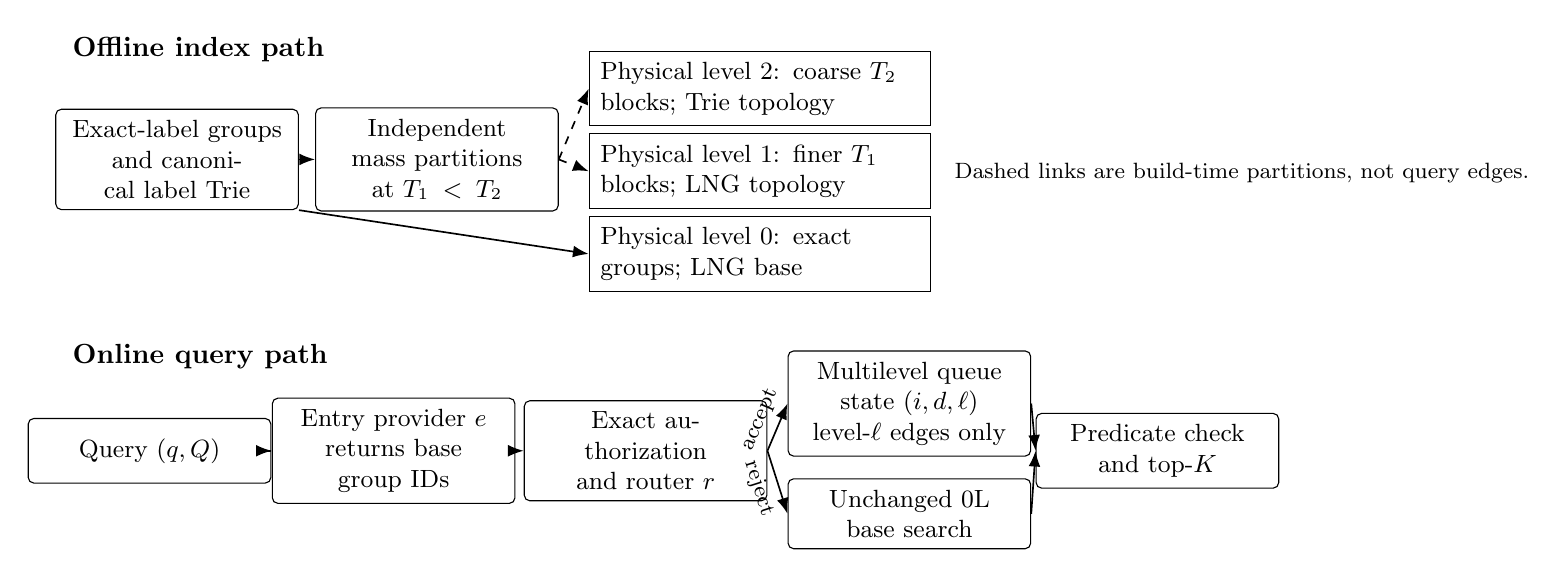
\begin{tikzpicture}[
  font=\small,
  box/.style={draw, rounded corners=2pt, align=center, minimum height=0.82cm,
              text width=2.8cm, inner sep=4pt},
  level/.style={draw, align=left, minimum height=0.72cm,
                text width=4.05cm, inner sep=4pt},
  flow/.style={-{Latex[length=2mm]}, semithick},
  build/.style={-{Latex[length=2mm]}, semithick, dashed}
]
\node[font=\bfseries, anchor=west] at (-0.2,1.75) {Offline index path};
\node[box] (groups) at (1.25,0.35) {Exact-label groups\\and canonical label Trie};
\node[box] (partition) at (4.55,0.35) {Independent mass partitions\\at $T_1<T_2$};
\node[level] (l2) at (8.65,1.25) {Physical level 2: coarse $T_2$ blocks; Trie topology};
\node[level] (l1) at (8.65,0.20) {Physical level 1: finer $T_1$ blocks; LNG topology};
\node[level] (l0) at (8.65,-0.85) {Physical level 0: exact groups; LNG base};
\draw[flow] (groups) -- (partition);
\draw[build] (partition.east) -- (l2.west);
\draw[build] (partition.east) -- (l1.west);
\draw[flow] (groups.south east) -- (l0.west);
\node[anchor=west, font=\footnotesize] at (11.0,0.18)
  {Dashed links are build-time partitions, not query edges.};

\node[font=\bfseries, anchor=west] at (-0.2,-2.15) {Online query path};
\node[box] (query) at (0.9,-3.35) {Query $(q,Q)$};
\node[box] (entry) at (4.0,-3.35) {Entry provider $e$\\returns base group IDs};
\node[box] (route) at (7.2,-3.35) {Exact authorization\\and router $r$};
\node[box] (multi) at (10.55,-2.75) {Multilevel queue\\state $(i,d,\ell)$\\level-$\ell$ edges only};
\node[box] (base) at (10.55,-4.15) {Unchanged 0L\\base search};
\node[box] (answer) at (13.7,-3.35) {Predicate check\\and top-$K$};
\draw[flow] (query) -- (entry);
\draw[flow] (entry) -- (route);
\draw[flow] (route.east) -- node[above,sloped,font=\footnotesize] {accept} (multi.west);
\draw[flow] (route.east) -- node[below,sloped,font=\footnotesize] {reject} (base.west);
\draw[flow] (multi.east) -- (answer.west);
\draw[flow] (base.east) -- (answer.west);
\end{tikzpicture}
\caption{\system architecture for the authoritative 2L-LT example.  Level 0,
level 1, and level 2 are three physical graphs.  The router chooses between
the multilevel backend and exact 0L fallback; inside the multilevel backend,
each state expands only edges owned by its tag.}
\label{fig:method-overview}
\end{figure*}

This separation also determines the ablations.  A 0L-Trie experiment changes
level-0 connectivity.  A Trie entry-provider experiment changes only the
initial frontier.  A 1L-versus-2L experiment adds level 2 while preserving the
level-1 partition.  These interventions are not labeled interchangeably.

\subsection{Predicate-Safe Coarsening by Trie Mass}
We build a canonical prefix trie over sorted group label sets.  Each terminal
stores one exact group and its point mass.  For a threshold $T_\ell$, a
bottom-up pass maintains uncovered mass.  When a non-root trie node has
uncovered mass greater than $T_\ell$, it becomes a block root and its uncovered
mass is reset before propagating upward.  The block owns terminal groups in its
subtree until another root at the same layer is encountered.  Each layer runs
this partition independently; adding a coarse layer therefore does not change
the blocks or identifiers of any finer layer.

For example, exact groups $\{a,b\}$, $\{a,c\}$, and $\{a,b,d\}$ can be direct
members of a block rooted at prefix $\{a\}$.  Query $Q=\{a\}$ authorizes this
block and may navigate the three groups at the coarser scale.  Query
$Q=\{a,b\}$ does not authorize the $\{a\}$ block, because
$Q\nsubseteq\{a\}$; it therefore uses a more specific authorized block or the
base graph.  The same containment test provides both predicate safety and
query-dependent scale selection without estimating selectivity.

\begin{algorithm}[t]
\caption{Independent block partition at threshold $T$}
\label{alg:partition}
\begin{algorithmic}[1]
\Require Canonical label trie $\mathcal{T}$ with terminal masses $w(v)$
\Ensure Disjoint direct-member blocks at one layer
\State $u(v)\gets w(v)$ for every trie node $v$
\For{nodes $v$ in reverse topological order}
  \State $u(v)\gets w(v)+\sum_{c\in\mathrm{child}(v)}u(c)$
  \If{$v$ is not the root and $u(v)>T$}
    \State emit a block rooted at $v$
    \State $u(v)\gets 0$
  \EndIf
\EndFor
\For{each emitted root $b$}
  \State assign terminals below $b$ until another emitted root is reached
\EndFor
\end{algorithmic}
\end{algorithm}

The build stores direct point count, full source-subtree count, common labels,
an entry point, and a nearest containing parent in the next coarser layer.  The
parent relation is metadata for inspection; query traversal does not use it to
promote candidates across layers.

\subsection{Layer-Local Topologies}
For each materialized layer, we support two group-to-group topologies.
\textbf{LNG} connects every block root to its minimal strict label supersets
within that layer.  \textbf{Trie} connects a terminal block to the nearest
terminal descendants along canonical prefix-trie branches.  Both point from a
less specific label set to a more specific one, but Trie is a strict sparsifier
and need not preserve every LNG reachability path.  We therefore treat its
quality as an empirical property, not a semantic equivalence.

Each block owns a local vector graph and vector-level inter-block edges.  Edges
are serialized with their owner block and activation level.  The base topology
is built independently and remains available for exact fallback.

Algorithm~\ref{alg:trie-topology} makes the Trie topology precise.  A preorder
scan carries the nearest terminal ancestor.  Consequently, every non-root
terminal has at most one incoming Trie edge and a terminal may have several
outgoing edges, one to the first terminal on each descendant branch.  The
result contains $O(G)$ edges, but unlike LNG it does not connect set-containment
relations whose sorted label sequences are not prefix related.  For a block
layer, terminals in the algorithm are the block roots emitted by
Algorithm~\ref{alg:partition}; traversal stops at the first nested block root,
so no edge crosses a layer boundary.

\begin{algorithm}[t]
\caption{Prefix-Trie group topology}
\label{alg:trie-topology}
\begin{algorithmic}[1]
\Require Canonical label trie $\mathcal{T}$ and terminals $g(v)$
\Ensure Directed topology $E_{\mathrm{Trie}}$
\State $E_{\mathrm{Trie}}\gets\varnothing$
\State push $(\mathrm{root}(\mathcal{T}),\bot)$ onto a stack
\While{the stack is nonempty}
  \State $(v,a)\gets\Call{Pop}{\mathrm{stack}}$
  \If{$v$ is a terminal}
    \If{$a\ne\bot$}
      \State $E_{\mathrm{Trie}}\gets E_{\mathrm{Trie}}\cup\{(g(a),g(v))\}$
    \EndIf
    \State $a\gets v$
  \EndIf
  \For{$c\in\mathrm{child}(v)$}
    \State push $(c,a)$ onto the stack
  \EndFor
\EndWhile
\State \Return $E_{\mathrm{Trie}}$
\end{algorithmic}
\end{algorithm}

\subsection{Entry-Group Providers}
The topology and the entry provider are separate interfaces.  The
\emph{original LNG} provider sorts and filters candidate supersets to return
the minimal observed supersets of $Q$.  The \emph{optimized LNG} provider
computes the same definition with label-cardinality buckets and indexed
containment checks.  The \emph{Trie} provider instead returns the first
compatible terminal on every surviving prefix branch.  It chooses the largest
query label as a pivot, enumerates only its posting list, verifies the remaining
labels by walking ancestors, and then descends each matched subtree until the
first terminal on each branch.  For $Q=\varnothing$, it returns the
precomputed root terminal frontier.  Thus all three providers return group
identifiers consumed by the same vector-search interface, but the Trie
frontier is deliberately topology aware and is not claimed to equal the LNG
minimal-superset set.

\subsection{Exact Authorization and Structural Eligibility}
A query authorizes block $b$ precisely when
\begin{equation}
  Q\subseteq R_b,
\end{equation}
where $R_b$ is the block root's sorted label set.  This test is independent of
estimated selectivity and observed latency.  Let $m$ be the coarsest
materialized overlay and let
\begin{equation}
  \mathcal{A}_m(Q)=\{b\mid \mathrm{level}(b)=m,\ Q\subseteq R_b\}.
\end{equation}
Because direct members partition each layer, the authorized direct mass
\begin{equation}
  M_m(Q)=\sum_{b\in\mathcal{A}_m(Q)} |P_b|
\end{equation}
does not count a point once at a coarse layer and again at a finer layer.

We distinguish two query-free routing policies. DRH-v1 executes the
multilevel backend whenever $\mathcal{A}_m(Q)$ is nonempty. DRH-v2 additionally
requires $M_m(Q)\ge T_{m+1}$, where $T_{m+1}$ is the next scale implied by the
same recurrence that constructs the $m$ upper overlays. If either test
fails, the router invokes the unchanged base-only algorithm before any overlay
seed is created. Otherwise all authorized overlays are eligible to seed the
multilevel search. Neither policy reads query frequencies, latency, Recall,
or a learned selectivity estimate.

\subsection{Level-Isolated Bounded Search}
Each candidate is a tuple $(i,d,\ell)$ containing a vector identifier, its
distance, and an activation level.  Level 0 denotes the base graph; level
$\ell>0$ denotes one materialized overlay.  Every authorized block contributes
its stored entry point, and entry groups contribute vector entry points tagged
with the level that owns them.  All seeds share one queue of capacity
$L_{search}$.

\begin{algorithm}[t]
\caption{Level-isolated multilevel query}
\label{alg:query}
\begin{algorithmic}[1]
\Require Query $(q,Q)$, entry provider $e$, hierarchy $H$, budget $L_s$,
optional mass threshold $T_{\mathrm{gate}}$
\State $B_Q\gets\{b\in H:Q\subseteq R_b\}$
\State $h\gets\max\{\mathrm{level}(b):b\in H\}$
\If{$B_Q$ has no block at level $h$}
  \State \Return \Call{BaseSearch}{$q,Q,e,L_s$}
\EndIf
\State $M_h\gets\sum_{b\in B_Q:\mathrm{level}(b)=h}|P_b|$
\If{$M_h<T_{\mathrm{gate}}$}
  \State \Return \Call{BaseSearch}{$q,Q,e,L_s$}
\EndIf
\State initialize a capacity-$L_s$ queue with block and entry-group seeds
\While{the queue has an unexpanded candidate $(i,d,\ell)$}
  \State pop the closest unexpanded candidate
  \If{$\ell=0$}
    \State $E\gets$ base edges of $i$
  \Else
    \State $E\gets$ edges of $i$ owned by level $\ell$
  \EndIf
  \For{$(i,j)\in E$}
    \If{the edge owner is authorized and $j$ is unseen at level $\ell$}
      \State insert $(j,\mathrm{dist}(q,x_j),\ell)$ into the bounded queue
    \EndIf
  \EndFor
\EndWhile
\State filter queue results by $Q$ and return the closest $K$
\end{algorithmic}
\end{algorithm}

There is no edge fallthrough, implicit promotion, or mixed-level expansion.
This provides a clean attribution of work to a layer.  It does not imply that
adding a layer is free: additional seeds can displace lower-layer candidates in
the shared bounded queue.

\subsection{Semantic Guarantees}
The hierarchy does not make approximate graph search exact, but its routing
and ownership rules provide three useful guarantees.

\paragraph{Authorization safety.}
If block $b$ is authorized, then every direct-member point of $b$ satisfies the
query predicate.  To see this, every member terminal is a descendant of the
block root and therefore contains all labels in $R_b$.  Authorization gives
$Q\subseteq R_b$, so transitivity yields $Q\subseteq A_i$ for every direct
member $i$ of $b$.  This claim is one-way: a block that is not authorized may
still contain some eligible points, which remain reachable through another
authorized layer or the base search.

\paragraph{Level-isolation invariant.}
Every expansion descended from a seed tagged $\ell$ scans only edges owned by
$\ell$.  The invariant holds initially because each seed is tagged with its
owning level.  During expansion, a special edge is accepted only when its owner
level equals the current tag, and its successor retains that tag; a level-0
candidate reads only base edges.  Induction over queue removals therefore
excludes both implicit promotion and fallthrough.  Separate visited sets per
level ensure that the same vector identifier in two layers does not collapse
the two search states.

\paragraph{Fallback equivalence.}
When the router rejects the overlay, the implementation invokes the same
base-search routine with the same entry provider, entry groups, and
$L_{search}$ as the corresponding 0L method. Under deterministic
execution, its returned neighbors and post-route search-work trace are
therefore identical. Total latency can still increase by the authorization
and mass tests themselves; we measure that cost rather than claiming that an
unused hierarchy is free.

\section{Calibration-Free Hierarchy Selection}
\subsection{Degree-Ratio Hierarchy}
DRH uses only values already required by index construction: $N$, maximum
within-layer degree $R$, and cross-block edge budget $C$.  We approximate the
cost of a first scale $T$ by
\begin{equation}
  \Phi(T)=T+\frac{N}{T},
\end{equation}
whose continuous minimizer is $\sqrt{N}$.  To stabilize discrete index layouts,
we round to the nearest power of two:
\begin{equation}
  T_1=2^{\left\lfloor \log_2\sqrt{N}+\frac{1}{2}\right\rfloor}.
\end{equation}
Successive thresholds use the existing degree ratio
\begin{equation}
  \rho=\max\left(2,\mathrm{round}\left(\frac{R}{C}\right)\right),
  \qquad T_{\ell+1}=\rho T_\ell.
\end{equation}
A scale is materialized while $N/T_\ell\ge C$.  Ignoring only the implementation
depth cap, the resulting number of upper overlays is therefore
\begin{equation}
  m=\max\left(0,
    1+\left\lfloor\log_\rho\frac{N}{C T_1}\right\rfloor\right).
\end{equation}
Thus the depth is derived, not configured separately.  The predeclared topology rule is LNG while the
estimated number of blocks exceeds one full local neighborhood and Trie near
the top:
\begin{equation}
  \tau_\ell=\begin{cases}
    \mathrm{LNG}, & N/T_\ell>R,\\
    \mathrm{Trie}, & \text{otherwise.}
  \end{cases}
\end{equation}
For the authoritative Amazon setup, $N=602{,}453$, $R=64$, and $C=4$, so DRH
selects $1024{:}\mathrm{LNG},16384{:}\mathrm{Trie}$ before examining query
performance. DRH-v2 sets its routing mass threshold to the next unmaterialized
scale,
\begin{equation}
  T_{\mathrm{gate}}=T_{m+1}=\rho T_m.
\end{equation}
This does not introduce an empirical knob: the value is already determined by
$N$, $R$, and $C$. DRH-v1, retained as an ablation, is equivalent to
$T_{\mathrm{gate}}=0$ with the nonempty-authorization requirement. We
emphasize that $\Phi$ and the mass gate are query-independent structural
proxies, not proofs of runtime optimality; held-out oracle regret tests whether
the complete policy transfers without query calibration.

The evaluated conservative single-base DRH instantiation treats level 0
differently from an overlay: it selects
$\tau_0=\mathrm{LNG}$ as the reachability anchor and applies the degree-ratio
rule only to $\ell>0$.  This is a policy choice rather than an implementation
restriction or an assumption of the method.
Tables~\ref{tab:base-topology-factorial-a}--\ref{tab:base-topology-factorial-b}
evaluate both possible bases with
all upper assignments.  The matched-provider 0L screen shows that Trie is
substantially faster at 0.5--5\%, but slower at 10\% and 60--99\%, and it does
not reach the Recall target at 30\% within the shared budget.  Overlays recover
that robustness and make several Trie-base systems the fastest measured
choices at both narrow and broad selectivities, but a static Trie-base choice
still loses to 0L LNG at 10--30\%.  Retaining LNG as the calibration-free base
therefore provides a conservative fallback; a dual-base query-time selector is
a useful extension, but is not silently folded into the reported policy.

\paragraph{Automation contract.}
This evaluated DRH policy therefore automates the number of upper overlays,
their thresholds and topologies, and the structural fallback gate.  It does
not claim that one base topology is optimal for every query regime.  The
complete factorial shows why: a Trie base is the strongest measured choice at
0.5--5\% and again after an effective coarse overlay is activated, whereas the
LNG base remains the strongest fallback at 10--30\%.  Selecting between two
materialized bases at query time would require an additional policy and its
own held-out validation; we leave that extension separate rather than deriving
it retrospectively from the Amazon outcomes.  Accordingly, our experimental
claims report both the full base-by-overlay design space and the narrower
calibration-free LNG-base DRH instantiation; they are not interchangeable.

\begin{algorithm}[t]
\caption{Degree-Ratio hierarchy with the DRH-v2 router}
\label{alg:drh}
\begin{algorithmic}[1]
\Require $N$, local degree $R$, cross-block degree $C$
\State $T\gets$ nearest power of two to $\sqrt{N}$
\State $\rho\gets\max(2,\mathrm{round}(R/C))$
\While{$N/T\ge C$}
  \State $\tau\gets\mathrm{LNG}$ if $N/T>R$, else $\mathrm{Trie}$
  \State append $(T,\tau)$ to the hierarchy plan
  \State $T\gets\rho T$
\EndWhile
\State $T_{\mathrm{gate}}\gets T$ \Comment{the next unmaterialized scale}
\State attach exact authorization and $M_h\ge T_{\mathrm{gate}}$ routing gate
\State \Return gated hierarchy plan
\end{algorithmic}
\end{algorithm}

Neither DRH variant is trained on query selectivity.  The frozen held-out
automatic-versus-manual comparison uses DRH-v1, because that candidate set was
pre-registered before the DRH-v2 routing ablation; the same-binary DRH-v2
results are reported separately and are not retroactively substituted into
the manual comparison.  Evaluation must
therefore separate the development dataset from held-out datasets and compare
it with both the best per-workload method and the best single manual
configuration used unchanged across workloads. Every held-out manual
configuration receives the same exact authorization gate, so oracle regret
measures only the cost of automatic depth, thresholds, and topology. Ungated
DRH is retained solely as an ablation.

\section{GPU-Assisted Construction}
\subsection{Irregular Construction Workload}
Index construction contains two different irregular workloads.  Intra-group
construction operates on many groups with a long-tailed size distribution.
Cross-group construction performs many $(n_q,n_x,d)\rightarrow\mathrm{topK}$
tasks induced by topology edges.  Launching a general GPU library once per
group or group pair repeats packing, transfer, launch, and writeback overhead.

\subsection{Base-Graph Pipeline}
The base index is constructed before any hierarchy sidecar.  Its pipeline has
four semantic stages: build a vector graph inside every exact-label group,
construct the group-to-group LNG, derive descendants and coverage, and
materialize vector-level cross-group edges.  Our optimization changes the
implementation of these stages, not their ownership: group topology and
metadata remain host structures, and the final vector adjacency is written in
the CPU-compatible index format used by search.

The accelerated group-graph path batches irregular exact-label groups and uses
the FastGrnnd CUDA candidate generator, followed by
relative-neighborhood-style pruning and configured degree repair.  The
cross-edge path converts host topology edges into descriptors for many
$(n_q,n_x,d)$ tasks.  A conventional GPU baseline computes similarity tiles
with SGEMM and performs top-$k$ as a separate stage.  Our fused path consumes
the descriptors directly, combines distance evaluation with group-local
top-$k$, and returns identifiers only because cross-edge distances are not
stored.  It keeps the base-vector array and norms resident when they fit the
declared device budget; otherwise, bounded vector and query chunks are
streamed.  Thus the optimization removes repeated per-pair invocation and
unnecessary score writeback without claiming a fully device-resident index
builder: host adjacency materialization remains an explicit measured
boundary.

\begin{algorithm}[t]
\caption{Accelerated construction of the base unified graph}
\label{alg:gpu-base-build}
\begin{algorithmic}[1]
\Require Vectors $X$, exact-label groups $\{G_S\}$, degree $R$, cross degree $C$
\Ensure CPU-compatible unified graph $A$
\State construct group metadata and the declared group topology
\For{each memory-bounded batch of exact-label groups}
  \State generate within-group candidates on the GPU
  \State prune candidates and repair each group to the declared degree policy
  \State append the resulting identifiers to host adjacency $A$
\EndFor
\State form descriptors $(G_S,G_{S'})$ for every group-topology edge
\For{each descriptor batch that fits the device budget}
  \State evaluate distances and select group-local top-$C$ identifiers jointly
  \State compact identifiers and append cross-group edges to $A$
\EndFor
\State execute the declared additional-edge completion path
\State serialize, reload, and validate $A$ and effective backend counters
\State \Return $A$
\end{algorithmic}
\end{algorithm}

Table~\ref{tab:base-build-profiles} freezes the five base-build profiles used
in the evaluation.  In particular, \texttt{naive\_gpu} and
\texttt{paper\_fused} retain CPU Vamana for intra-group graphs, isolating the
cross-edge kernel change; \texttt{accelerated\_\allowbreak gpu} additionally selects the
CUDA group-graph implementation, optimized metadata, and the configured CPU
exact-scan additional-edge path.

\begin{table*}[t]
\caption{Frozen base-graph construction profiles.  ``Optimized metadata''
denotes bucketed minimal-superset discovery, optimized LNG construction,
epoch-based descendants, and direct descendant coverage.}
\label{tab:base-build-profiles}
\centering
\scriptsize
\begin{tabular}{p{0.13\textwidth}p{0.19\textwidth}p{0.25\textwidth}p{0.32\textwidth}}
\toprule
Profile & Intra-group graph & Group metadata & Vector cross-group edges \\
\midrule
\texttt{original\_cpu} & CPU Vamana & Original sort/LNG, hash-BFS descendants, topological coverage & Original CPU builder \\
\texttt{current\_cpu} & CPU Vamana & Optimized metadata & CPU Vamana cross-edge builder \\
\texttt{naive\_gpu} & CPU Vamana & Optimized metadata & Batched GPU SGEMM plus separate top-$k$ \\
\texttt{paper\_fused} & CPU Vamana & Optimized metadata & Descriptor-grouped fused distance/top-$k$ with identifier-only writeback \\
\texttt{accelerated\_gpu} & FastGrnnd CUDA path & Optimized metadata & Fused GPU cross edges plus CPU exact-scan additional edges \\
\bottomrule
\end{tabular}
\end{table*}

\subsection{Hierarchy Intra-Block Graphs}
For each hierarchy layer, the intra-block router sends small blocks to CPU
exact top-$k$ (or bounded
complete) graphs, medium blocks to sampled CPU Vamana
construction~\cite{subramanya2019diskann}, and large blocks to a GPU adaptation
of NN-Descent candidate generation~\cite{dong2011nndescent} followed by
relative-neighborhood-style pruning~\cite{toussaint1980rng} and degree repair.
The authoritative configurations use
$n_{\mathrm{small}}=2048$, $n_{\mathrm{large}}=8192$, and 256 sampled
candidates for the middle route.  These fixed construction settings are shared
by the compared hierarchy structures and are not inputs to DRH.  A separate
full-GPU profile disables this three-way router and sends every block above the
small-block completion threshold to the CUDA path.  Routing is determined by
block cardinality and does not inspect downstream Recall.  GPU output is
compacted before device-to-host transfer, but the current system still
materializes CPU-compatible adjacency lists.  We report that conversion as an
output-boundary cost rather than kernel work, and record any CUDA failure that
falls back to CPU.

\subsection{Grouped Fused Cross-Block Top-$k$}
For every topology edge, source vectors need nearest target vectors.  The GPU
path groups descriptors across irregular tasks, keeps base vectors resident
when capacity permits, addresses queries by global vector identifier, fuses
distance and top-$k$ selection, and writes identifiers only when distances are
not consumed downstream.  This design builds on GPU similarity-search work
that identifies $k$-selection and memory traffic as central
bottlenecks~\cite{johnson2021gpu}.  Large workloads use bounded streaming
rather than assuming that the full vector array fits device memory.  CPU
fallback remains explicit and is recorded in build logs.

Algorithm~\ref{alg:gpu-build} gives the end-to-end sidecar path.  The routing
decision depends only on block cardinality and declared memory limits.  In
particular, a GPU-labelled result is invalid when a requested GPU stage falls
back silently; our validator checks the effective backend counters persisted
by the builder.

Intra-block and inter-block execution are independently controlled.  We
therefore freeze the five hierarchy profiles in
Table~\ref{tab:hierarchy-build-profiles}, rather than describing a sidecar with
one undifferentiated GPU switch.  The \texttt{full\_gpu} profiles disable the
three-way intra router and send every block above the bounded-complete
threshold to CUDA.  The WMMA variant changes the inter-block fused top-$k$ to
TF32 tensor-core execution; it does not redefine the hierarchy or the
intra-block graph algorithm.

\begin{table*}[t]
\caption{Frozen hierarchy-sidecar construction profiles.  CPU completion is
retained below the declared small-block threshold in every profile.}
\label{tab:hierarchy-build-profiles}
\centering
\scriptsize
\begin{tabular}{p{0.18\textwidth}p{0.35\textwidth}p{0.34\textwidth}}
\toprule
Profile & Intra-block route & Inter-block route \\
\midrule
\texttt{cpu} & Small exact/complete, medium sampled Vamana, large CPU Vamana & CPU \\
\texttt{hybrid\_gpu\_intra} & Small exact/complete, medium sampled Vamana, large FastGrnnd-style CUDA & CPU \\
\texttt{hybrid\_gpu\_intra\_inter} & Same hybrid intra route & Fused CUDA top-$k$ \\
\texttt{full\_gpu} & Bounded completion, then CUDA & Fused CUDA-core top-$k$ \\
\texttt{full\_gpu\_wmma} & Bounded completion, then CUDA & Fused TF32-WMMA top-$k$ \\
\bottomrule
\end{tabular}
\end{table*}

\begin{algorithm}[t]
\caption{Hybrid GPU construction of a multilevel sidecar}
\label{alg:gpu-build}
\begin{algorithmic}[1]
\Require base vectors $X$, label trie $\mathcal{T}$, layer plan
  $\{(T_\ell,\tau_\ell)\}$, degree $R$, cross-edge budget $C$, device budget $M$
\Ensure validated CPU-compatible sidecar and backend evidence
\For{each layer $\ell$ independently}
  \State $\mathcal{B}_\ell\gets\Call{PartitionTrie}{\mathcal{T},T_\ell}$
  \State $\mathcal{E}_\ell\gets\Call{BuildTopology}{\mathcal{B}_\ell,\tau_\ell}$
  \For{each block $b\in\mathcal{B}_\ell$}
    \If{$|b|\le n_{\mathrm{small}}$}
      \State $A_b\gets\Call{ExactTopKCPU}{X_b,R}$
    \ElsIf{$|b|<n_{\mathrm{large}}$}
      \State $A_b\gets\Call{SampledVamanaCPU}{X_b,R}$
    \Else
      \State $C_b\gets\Call{GPUCandidateGraph}{X_b,M}$
      \State $A_b\gets\Call{RNGPruneAndRepair}{C_b,R}$
    \EndIf
  \EndFor
  \State $\mathcal{P}\gets\{(u,v):(u,v)\in\mathcal{E}_\ell\}$
  \For{each memory-bounded descriptor batch $P\subseteq\mathcal{P}$}
    \State $A_P\gets\Call{FusedDistanceTopK}{X,P,C,M}$
    \State compact identifiers and append $A_P$ to layer-local adjacency
  \EndFor
  \State record GPU work, explicit CPU fallbacks, phase times, and edge counts
\EndFor
\State serialize, reload, and structurally validate every declared layer
\State \Return sidecar and effective-backend evidence
\end{algorithmic}
\end{algorithm}

Layer-local and inter-block edges have independent backend choices, while all
layers within a named profile use the same declared routing policy.  A case is
accepted only if its log proves the requested GPU work occurred, reports zero
GPU intra-block fallback, proves GPU inter-block use when requested, and, for
\texttt{full\_gpu\_wmma}, contains an observed \texttt{mode=tf32\_wmma}
execution.  We then serialize and reload every declared layer and validate its
structure.  A predeclared quality cohort additionally re-queries the original
and accelerated base indexes and the CPU, full-GPU, and full-GPU-WMMA
sidecars for both studied hierarchy structures under the same formal
equal-Recall protocol as the query study.  Backend evidence is therefore
necessary but not sufficient for a claimed construction result.

Because the hierarchy is an independent sidecar, its total build time satisfies
\begin{equation}
  T_{\mathrm{multilevel}}=T_{\mathrm{base}}+T_{\mathrm{sidecar}}.
\end{equation}
We therefore compare total multilevel build against the original CPU build,
and report sidecar overhead against the same accelerated base separately.

\section{Complexity Analysis}
Let $G$ be the number of exact groups, $B_\ell$ the number of blocks at layer
$\ell$, $G_\ell$ the number of exact-group memberships assigned at that layer,
$M_\ell$ the number of direct member points represented at that layer,
$E_\ell$ its block-topology edges, and $D_\ell$ the number of materialized
vector edges.  Building the label trie costs $O(\sum_g |S_g|)$ time and space.
Each independent partition is linear in the trie plus emitted memberships, so
all partitions cost
\begin{equation}
  O\left(L|\mathcal{T}|+\sum_{\ell=1}^{L}G_\ell\right).
\end{equation}
The stored hierarchy costs $O(\sum_\ell(B_\ell+G_\ell+D_\ell))$ excluding the
base index.  Trie topology has one incoming nearest-terminal edge per
non-root terminal and hence $O(B_\ell)$ block edges, whereas explicit LNG
construction can require pairwise containment checks and a denser transitive
reduction in the worst case.  We report the materialized edge counts rather
than infer cost from these bounds.

For one query, exact block authorization by direct comparison is
$O(\sum_b |R_b|)$; indexed Trie search can reduce the examined frontier, but we
report measured authorization time rather than assuming a distribution.
Bounded graph search stores $O(L_{search})$ candidates.  Its dominant time is
\begin{equation}
  O\left(D_q d + I_q\log L_{search}\right),
\end{equation}
where $D_q$ is the measured number of distance computations and $I_q$ is the
number of successful queue insertions.  Since multiple authorized layers share
the queue, neither quantity is guaranteed to decrease with depth.

\section{Experimental Methodology}
\subsection{Questions}
We ask: (Q1) When does multiscale navigation improve over the single-scale
UNG structure at equal Recall? (Q2) Which effects come from topology, entry
discovery, and hierarchy depth? (Q3) How close is DRH to manual tuning on
development and held-out datasets? (Q4) Can GPU assistance keep total
multilevel construction competitive with the original CPU pipeline? (Q5)
Which phase and work counters explain each result?

\subsection{Datasets and Workloads}
The development dataset is Amazon with $602{,}453$ vectors of dimension 768 and
$482{,}387$ observed label groups.  Each workload contains 1,000 queries, uses
$K=10$, and has exact containment ground truth.  The measured mean
selectivities are 0.499249\%, 0.903055\%, 5.038117\%, 9.906615\%, 30.027242\%,
60.047491\%, 80.023699\%, 95.019781\%, and 99.000600\%.  Genome, Reviews, and
VariousImg are held out for the automatic-policy study; their exact workload
directories and fingerprints are recorded in the artifact manifest.
\authoritativeDatasetTable
The 99\% Amazon workload contains 697 empty predicates and 303 singleton
predicates $\{1\}$.  We retain this mixture because both are legal containment
queries, and validate the empty-predicate path separately before timing.

\subsection{Methods and Fairness}
The principal 0L comparison is LNG topology with optimized-LNG entry
discovery versus Trie topology with Trie entry discovery.  The topology
factorial fixes $T_1=1024$, $T_2=16384$, and ungated routing while enumerating
both base topologies and every LNG/Trie upper-layer assignment through 2L.
Within either base, replacing one upper letter is a controlled topology
comparison because its entry provider is unchanged.  Across bases we instead
report a matched-provider system comparison, not a pure edge-topology effect.
A separate compatibility ablation crosses the three legal entry strategies
(original LNG, optimized LNG, and Trie) with selected topologies.  Routed
controls are outside the factorial because routing changes which search
algorithm executes. For held-out automatic-policy evaluation, however,
the exact gate is fixed for DRH and every manual-alternative hierarchy; the
ungated DRH variant is reported separately.

We call the 0L LNG configuration \emph{Plain} or \emph{0L-LNG}.  It
preserves UNG's exact-label groups, LNG cover relation, and unified vector
graph, but it is not the unmodified upstream release: it uses our optimized,
semantically equivalent minimal-superset provider and the common refactored
execution path.  This is the stronger control for the hierarchy because Plain
and every overlay method share entry discovery and base-graph code.  Reported
multilevel speedups therefore isolate navigation scale; they are not presented
as direct timings against the original UNG binary.

All query methods use the same data, query vectors, labels, exact ground truth,
$K$, thread count, immutable search binary, graph backend, and Recall protocol.
\authoritativeQueryExecution
Every repeat executes the same frozen query file in the same order; repeats are
repeated measurements, not new random samples.  We discard the cold repeat,
derive primary QPS from the median warm batch time, and retain per-repeat values
for dispersion estimates.  Recall is not averaged to relax the quality target:
every warm repeat at the selected operating point must meet the threshold.
We select the smallest \emph{measured} $L_{search}$ for which every warm repeat
reaches Recall@10 $\ge0.90$; there is no interpolation or extrapolation.  The
screen pass locates crossings and a separate profile pass collects expensive
counters. The current deadline artifact uses one discarded cold repeat and two
warm repeats; a later formal pass is reserved for confidence intervals. If a method has no screen crossing, its
crossing pass extends to the largest $L_{search}$ measured for any method on
that workload (or an explicitly declared common cap); only failure at that
shared budget is reported as no crossing.
\authoritativeSharedSearchBudgetTable

\subsection{Metrics}
Table~\ref{tab:metric-definitions} defines every quantity used in the query
tables.  The batch size is $B=1000$ queries.  Primary query metrics are
warm-median batch latency and QPS. Bootstrap 95\% confidence intervals are
reserved for the later formal pass and are not claimed by the current deadline
artifact.

\begin{table*}[t]
\caption{Measurement definitions.  A ``warm median'' is taken across the two
warm repeats in the current screen-level artifact; it is not a confidence
interval.  Per-query stage times and work counters are first averaged over all
queries in one repeat and then summarized across warm repeats.}
\label{tab:metric-definitions}
\centering
\small
\begin{tabular}{p{0.19\textwidth}p{0.73\textwidth}}
\toprule
Reported quantity & Definition \\
\midrule
Mean selectivity & $B^{-1}\sum_{j=1}^{B}|\eligible(Q_j)|/N$ for the frozen query batch; it describes the workload and is not an input to DRH. \\
Recall@10 & For one repeat, the mean over queries of $|R_{10}(q_j,Q_j)\cap R^*_{10}(q_j,Q_j)|/10$.  A crossing requires every warm repeat at that executed point to reach 0.90. \\
$L_{search}$ & Capacity of the bounded candidate queue.  An equal-Recall operating point is the smallest executed $L_{search}$ that crosses the Recall target; values between executed points are not interpolated. \\
Batch latency / QPS & Wall time to complete all $B$ queries with 100 query threads, after the cold repeat is discarded; $\mathrm{QPS}=1000B/\mathrm{batch\ latency\ (ms)}$. \\
$A/B$ speedup & $\mathrm{QPS}_A/\mathrm{QPS}_B$, using each method's selected equal-Recall crossing.  A ratio above one favors $A$. \\
NC / $R_{\max}$ & NC means no Recall crossing within the workload-wide measured $L_{search}$ budget.  $R_{\max}$ is the largest minimum-over-warm-repeats batch Recall observed in that budget. \\
ELS / entry / authorization & Mean milliseconds per query for Entry Label Set (entry-group) discovery, vector entry-point setup, and exact block-authorization plus routing work, respectively. \\
Graph / residual & Mean milliseconds per query inside bounded graph traversal, and the remaining measured query time outside the named stages. \\
Visited / edges / distances & Mean per-query counts of popped graph states, scanned adjacency entries, and vector-distance evaluations.  Base and overlay edges are counted separately where enabled. \\
\bottomrule
\end{tabular}
\end{table*}

Build results use process wall time through validated files on disk. The full protocol requires one cold build followed by at least five
measured builds, interleaved CPU/GPU order, and peak host/device memory in a separate
pass, and index bytes.  Full-index cost is the sum of independently measured
base and hierarchy stage medians; confidence intervals independently resample
all three stages rather than pairing repeat identifiers across phases.  GPU
kernel timings are never substituted for construction wall time. GPU runs use an external
exclusive lock when the host provides one.  On the current host, where that
tool is unavailable, each GPU case instead requires three consecutive idle
device snapshots before timing; we retain those snapshots and label the
result as an idle-preflight measurement rather than claiming lock-level
exclusivity.  The completed construction study reports two measured timing
repeats per hierarchy backend and a separate resource pass.  Its composed
base-plus-hierarchy result sums independently measured stage medians and is
explicitly distinguished from a single jointly timed build.

\section{Results}
\authoritativeResults
\baseTopologyFactorialTables
\baseTopologyFactorialFindings
\authoritativeRecallQPSFigures

\section{Discussion}
\subsection{Why More Layers Are Not Monotone}
Level isolation prevents an upper candidate from scanning lower-level edges,
but does not make an extra layer cost-free.  Authorized block seeds enter the
same bounded queue as base or finer-layer seeds.  They consume distance
computations and can displace candidates before useful regions are expanded.
DRH-v1 removes this overhead only for queries that authorize no upper block.
DRH-v2 also rejects an authorized overlay whose highest-layer direct mass is
below the next hierarchy scale. This remains a structural rule rather than a
latency predictor, so it cannot guarantee that every accepted overlay is
profitable.

\subsection{Trie Topology Is a Sparsifier, Not an LNG Alias}
Canonical prefix adjacency is cheaper and can be highly effective when query
entries align with its branches.  It omits non-prefix subset relations,
however, so increasing $L_{search}$ is not guaranteed to expose every region
from a fixed entry frontier before the search becomes effectively exhaustive.
This also explains why crossing an LNG-style minimal-superset entry frontier
with a Trie topology can reduce work yet lower Recall: fewer seeds do not cover
every prefix branch retained by the Trie graph.  A full-budget run can still
cross by exhausting most candidates, which is correctness evidence but not an
efficient operating point.  We therefore report no-crossing outcomes within
the shared budget explicitly and pair Recall with entry count, visited-node,
scanned-edge, and distance-computation counts.

\subsection{Limitations}
DRH uses a symmetric static cost proxy, existing degree budgets, exact
authorization, and a next-scale mass gate; it does not use a learned cost model
or query frequencies. The
held-out study is required to distinguish genuine structural generalization
from an Amazon-specific coincidence.  The GPU pipeline retains a host
adjacency materialization boundary, and full device-resident construction is
future work.  All four evaluated datasets instantiate two upper DRH overlays
(2L), so the
held-out study tests transfer of thresholds and topology but does not by itself
establish performance when the derived depth changes.  Finally, the current
evaluation covers containment predicates;
other predicate semantics require a new authorization proof.

\section{Related Work}
\subsection{Filtered Graph Search and UNG}
Graph-based ANN systems such as HNSW~\cite{malkov2020hnsw} and
DiskANN~\cite{subramanya2019diskann} use navigable proximity graphs to obtain
high-recall search with bounded expansion.  Filtered-DiskANN~\cite{gollapudi2023filtereddiskann}
and ACORN~\cite{patel2024acorn} integrate metadata constraints through
filter-aware construction or predicate-agnostic graph expansion.

Range-filtered systems expose a related granularity problem in an ordered
attribute domain.  SeRF compresses range-dedicated graphs into segment
graphs~\cite{zuo2024serf}; iRangeGraph composes a query-time graph from
materialized elemental ranges~\cite{xu2024irangegraph}; and UNIFY supports
pre-, post-, and hybrid filtering from a segmented inclusive
graph~\cite{liang2024unify}.  Subsequent work extends range-specialized
structures to streaming arrivals and efficient updates
~\cite{peng2025dynamic,zhang2025rangepq}.  These systems motivate making
granularity explicit, but their interval decompositions do not directly solve
set containment: label sets form a partial order, and prefix adjacency does
not contain every subset edge.

UNG~\cite{cai2024ung} is our closest baseline.  Its contribution is an LNG
whose vertices are observed exact label sets and whose edges encode minimal
strict-superset relations; group-level relations are then realized in one
unified vector graph.  \system does not replace this containment abstraction.
It retains it at level zero and adds independently partitioned block overlays
above it.  Authorization follows from the common labels at a block root, and a
level tag restricts each expansion to one overlay.  This is also distinct from
HNSW's hierarchy: HNSW samples vector vertices to accelerate geometric
navigation, whereas our layers aggregate label-space regions and are selected
by an exact predicate test.  Prefix-Trie connectivity is an optional
inter-block sparsifier in our framework, not a relabeling of UNG's existing
Trie-assisted entry lookup.

Recent systems make workload heterogeneity itself an index-design concern.
Elastic Index Selection exploits containment among label sets to choose and
share partial indexes under an elastic-factor bound
~\cite{yang2025elastic}.  Curator advocates a dual-index architecture for the
low-selectivity regime and shares label-specialized indexes through a
clustering tree~\cite{jin2026curator}.  Their conclusions reinforce our
factorial result that no single organization should be presumed best across
all filter regimes.  Our focus is complementary: we study independently
materialized navigation scales inside one containment-oriented graph system,
make LNG-versus-Trie topology a per-level choice, and derive a query-trace-free
hierarchy plan.  We do not claim that DRH replaces workload-aware index
selection; the held-out VariousImg counterexample demonstrates that boundary.

\subsection{Graph Construction}
NN-Descent~\cite{dong2011nndescent} provides an efficient iterative basis for
approximate $k$-NN graph construction, while relative neighborhood
graphs~\cite{toussaint1980rng} motivate diversity-oriented proximity pruning.
Recent database work attacks construction cost through tree/graph hybrids,
LSH-assisted insertion, monotonic neighborhoods, or revised pruning
~\cite{azizi2023elpis,zhao2023lshapg,peng2023taumng,yang2025pgbuild}.
Starling instead co-designs an in-memory navigator, disk layout, and block
search for I/O efficiency~\cite{wang2024starling}.  GPU similarity search
supplies high-throughput distance and top-$k$ primitives~\cite{johnson2021gpu},
but per-group invocation can be dominated by packing and launch overhead.  Our
construction contribution is narrower: it batches the many irregular
intra-block and cross-block tasks of a predicate hierarchy while preserving
the CPU-compatible adjacency format.  We therefore report both stage time and
composed full-index wall time rather than equating a fast kernel with a fast
builder.

\section{Conclusion}
UNG established exact-label groups and containment-directed cross-group edges
as a unified substrate for filtered graph search.  \system addresses the next
bottleneck: one exact-group navigation scale cannot efficiently serve every
eligible mass.  Predicate-safe Trie blocks provide coarse overlays while the
original group graph remains level zero.  Exact authorization and level-local
edges make this multiscale behavior auditable, and DRH derives depth,
thresholds, topology, and routing without query calibration.  The accompanying
protocol evaluates measured Recall crossings and separates kernel, component
wall time, and stage-composed full-index construction costs.
\authoritativeConclusionResult

\authoritativeScreenAppendix

\bibliographystyle{ACM-Reference-Format}
\bibliography{references}

\end{document}
